\documentclass[11pt,a4paper]{article}

\usepackage[utf8]{inputenc}
\usepackage[T1]{fontenc}
\usepackage[brazil]{babel}
\usepackage[margin=2.5cm]{geometry}
\usepackage{graphicx}
\usepackage{array}
\usepackage{booktabs}
\usepackage{amsmath}
\usepackage{gensymb}
\usepackage{xcolor}
\usepackage{listings}
\usepackage{float}
\usepackage{caption}
\usepackage{enumitem}
\usepackage[colorlinks=true,linkcolor=blue!50!black,citecolor=blue!50!black,urlcolor=blue!40!black]{hyperref}
\usepackage[backend=biber,style=numeric,sorting=none]{biblatex}
\addbibresource{referencias.bib}
\usepackage{pdfpages}

\lstset{
  basicstyle=\ttfamily\small,
  breaklines=true,
  columns=fullflexible,
  backgroundcolor=\color{black!5},
  frame=single,
  framesep=3pt,
  xleftmargin=3pt,
  xrightmargin=3pt,
}

\newcommand{\todolink}[1]{\textcolor{red}{\textbf{[TODO: #1]}}}

\title{
  \Large Análise de Tabuleiros de Xadrez\\
  \large Visão Computacional Clássica e Transfer Learning para Leitura Completa de Partidas\\[0.5em]
  \normalsize Relatório Final --- INE410121 / TRV410001 --- Visão Computacional --- UFSC
}
\author{Davi Ludvig \and Julia Macedo}
\date{Julho de 2026}

\begin{document}

\maketitle

\begin{abstract}
\noindent
Este relatório descreve uma pipeline de visão computacional para leitura automática de
tabuleiros de xadrez fotografados em perspectiva, combinando técnicas clássicas de
processamento de imagens (suavização, detecção de bordas, Transformada de Hough,
homografia, votação de características) com \textit{deep learning} (\textit{transfer
learning} e \textit{fine-tuning} de uma ResNet-34) para a etapa de classificação do tipo
de peça. A solução cobre o problema de ponta a ponta: da imagem bruta até a
reconstrução da posição em notação FEN e a inferência de jogadas (incluindo capturas,
roque, \textit{en passant} e promoção). São reportadas métricas quantitativas para cada
etapa --- detecção de ocupação, classificação de cor, classificação de tipo de peça e
leitura de ponta a ponta --- avaliadas sobre o dataset \textit{Synthetic Chess Board
Images} (Kaggle). O gargalo identificado é a detecção automática dos cantos do
tabuleiro; isolando esse erro, o F1 de ocupação sobe de 62,7\% para 86,3\%, enquanto o
classificador de tipo de peça atinge F1 de 91\%.
\end{abstract}

\tableofcontents
\newpage

\section{Introdução}

\subsection{Motivação e contexto}

A digitalização automática de partidas de xadrez a partir de imagens tem aplicações
práticas relevantes: transmissão de torneios (conversão de uma partida física em
notação digital, em tempo real, sem sensores no tabuleiro), alimentação de
\textit{engines} de análise a partir da posição capturada por câmera, acessibilidade
(descrição automática de uma partida para pessoas com deficiência visual), e como
estudo de caso para o ensino de Visão Computacional --- o tabuleiro combina geometria
regular e previsível com uma quantidade significativa de variabilidade visual (ângulo de
câmera, iluminação, material das peças).

Este projeto foi desenvolvido para a disciplina INE410121 / TRV410001 --- Visão
Computacional (UFSC) e tem como objetivo construir, do zero, uma pipeline completa de
leitura de tabuleiro: da fotografia bruta em perspectiva até a notação FEN da posição e
a identificação da jogada realizada entre dois estados consecutivos do tabuleiro.

\subsection{Por que uma abordagem híbrida (clássica + \textit{deep learning})}

A disciplina é centrada em técnicas clássicas de processamento de imagens --- domínio do
valor (histogramas, limiarização), domínio do espaço (operadores de borda, suavização,
morfologia), geometria projetiva (Hough, homografia) --- e a maior parte da pipeline
deste trabalho é resolvida com essas ferramentas. A exceção deliberada é a
\textbf{classificação do tipo de peça} (peão, torre, cavalo, bispo, dama, rei), etapa em
que abordagens clássicas (\textit{template matching}, momentos de Hu, HOG) mostraram-se
insuficientes: as doze classes de peça, fotografadas em ângulo e talhadas no mesmo
material do tabuleiro, produzem silhuetas ambíguas demais para descritores clássicos de
forma. Nessa única etapa, o projeto recorre a \textit{transfer learning} com uma
ResNet-34 pré-treinada, mantendo clássica toda a geometria (detecção de bordas, linhas,
homografia, segmentação) e a decisão de ocupação/cor.

Essa escolha não é apenas prática --- ela também é didaticamente interessante: o
resultado final expõe, lado a lado, onde a visão clássica é suficiente (leitura
geométrica do tabuleiro) e onde ela deixa de ser competitiva (reconhecimento de forma
fina sob baixo contraste), permitindo comparar diretamente o custo/benefício das duas
famílias de técnicas sobre o mesmo problema.

\subsection{Objetivos}

\begin{enumerate}[nosep]
  \item Detectar automaticamente o tabuleiro em uma foto em perspectiva e corrigir a
        distorção via homografia, obtendo uma vista de cima (\textit{top-down}).
  \item Segmentar o tabuleiro retificado em 64 casas e determinar, para cada uma, se
        está ocupada e, em caso positivo, a cor da peça.
  \item Classificar o tipo de cada peça ocupante via \textit{transfer learning}.
  \item Reconstruir a posição completa em notação FEN (todos os seis campos).
  \item Comparar dois estados consecutivos do tabuleiro e inferir a jogada realizada,
        incluindo casos especiais (captura, roque, \textit{en passant}, promoção).
  \item Quantificar o desempenho de cada etapa isoladamente e da pipeline de ponta a
        ponta, identificando o gargalo do sistema.
\end{enumerate}

\subsection{Organização do documento}

A Seção~\ref{sec:dataset} descreve o dataset utilizado. A
Seção~\ref{sec:metodologia} detalha a pipeline clássica (pré-processamento, bordas,
Hough, homografia, segmentação, ocupação e cor). A Seção~\ref{sec:deep-learning} cobre o
classificador de tipo de peça baseado em ResNet-34. A Seção~\ref{sec:fen-jogadas}
descreve a reconstrução de FEN e a detecção/notação de jogadas. A
Seção~\ref{sec:resultados} apresenta os resultados quantitativos de cada etapa e da
leitura de ponta a ponta. A Seção~\ref{sec:limitacoes} discute limitações conhecidas e
trabalhos futuros, seguida da conclusão e dos links de referência do projeto.

\section{Dataset}
\label{sec:dataset}

O projeto utiliza o dataset público \textbf{Synthetic Chess Board Images}
\cite{dataset-chess}, disponível no Kaggle sob licença CC0 (domínio público). Suas
características principais:

\begin{itemize}[nosep]
  \item \textbf{Volume:} aproximadamente 1\,900 imagens de tabuleiros fotografados em
        ângulo (não \textit{top-down}), resolução $1280 \times 1280$ pixels, formato
        JPEG.
  \item \textbf{Material:} tabuleiro e peças de madeira (\textit{boxwood} para peças
        claras, \textit{ebony} para escuras), o que produz baixo contraste entre peça e
        fundo em diversas condições de iluminação.
  \item \textbf{Anotações:} um arquivo JSON por imagem contendo (a) a configuração da
        posição --- \texttt{config} --- mapeando cada casa ocupada ao tipo e cor da
        peça, e (b) os quatro cantos do tabuleiro --- \texttt{corners} --- normalizados
        no intervalo $[0,1]$ (multiplicados pelas dimensões da imagem para obter
        coordenadas em pixels).
  \item \textbf{Superfícies, iluminação e ângulos de câmera variados} entre as imagens,
        o que exige que a detecção de cantos e a classificação de ocupação/cor
        generalizem além de um único cenário fixo.
\end{itemize}

O dataset não contém sequências de jogo contínuas --- cada imagem é uma posição
independente, gerada separadamente. Isso é relevante para a Seção~\ref{sec:fen-jogadas}:
a validação do detector de jogadas é feita com posições controladas (montadas
manualmente) e não com transições reais capturadas entre dois instantes do mesmo
tabuleiro.

\subsection{Download e uso}

O dataset é obtido programaticamente via \texttt{kagglehub} e fica em cache local em
\texttt{\textasciitilde/.cache/kagglehub/}; o projeto não versiona os dados brutos. O
bootstrap de ambiente (local ou Google Colab) e o download automático estão
implementados em \texttt{src/setup.py} do repositório do projeto (ver
Seção~\ref{sec:links}).

\section{Pipeline Clássica: da Imagem ao Mapa de Ocupação}
\label{sec:metodologia}

A Figura~\ref{fig:pipeline-overview} resume as etapas descritas nesta seção: da imagem
bruta à obtenção de um mapa de ocupação e cor por casa. Todas as etapas usam apenas
técnicas clássicas de processamento de imagens.

\begin{figure}[H]
  \centering
  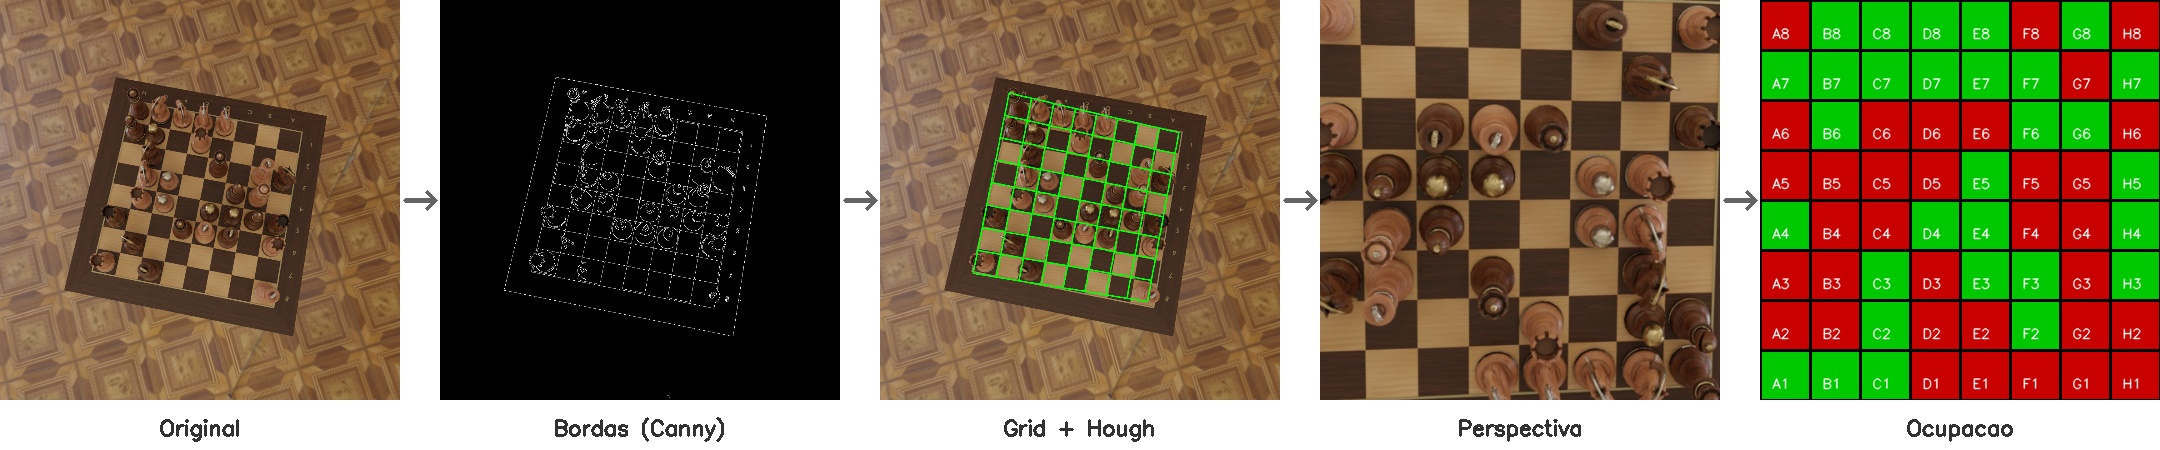
\includegraphics[width=0.85\textwidth]{../../intro/images/slide_pipeline.jpg}
  \caption{Visão geral da pipeline clássica: bordas, linhas de Hough, homografia,
    segmentação 8$\times$8, votação de características.}
  \label{fig:pipeline-overview}
\end{figure}

\subsection{Pré-processamento}

A imagem é convertida para tons de cinza usando a luminância perceptual do OpenCV
(\texttt{COLOR\_BGR2GRAY}), $Y = 0{,}114B + 0{,}587G + 0{,}299R$, pois a maioria dos
operadores de borda opera sobre imagens monocromáticas. Em seguida aplica-se suavização
gaussiana (kernel $5\times5$, $\sigma$ calculado automaticamente pelo OpenCV) para
reduzir ruído de alta frequência antes da detecção de bordas --- ruído gera gradientes
espúrios que se traduzem em bordas falsas.

Histograma de intensidade, equalização global (\texttt{equalizeHist}) e CLAHE
(\texttt{clipLimit=2.0}, \texttt{tileGridSize=(8,8)}) foram usados como ferramentas de
diagnóstico da distribuição de intensidade do dataset, mas não fazem parte da pipeline
principal.

\begin{figure}[H]
  \centering
  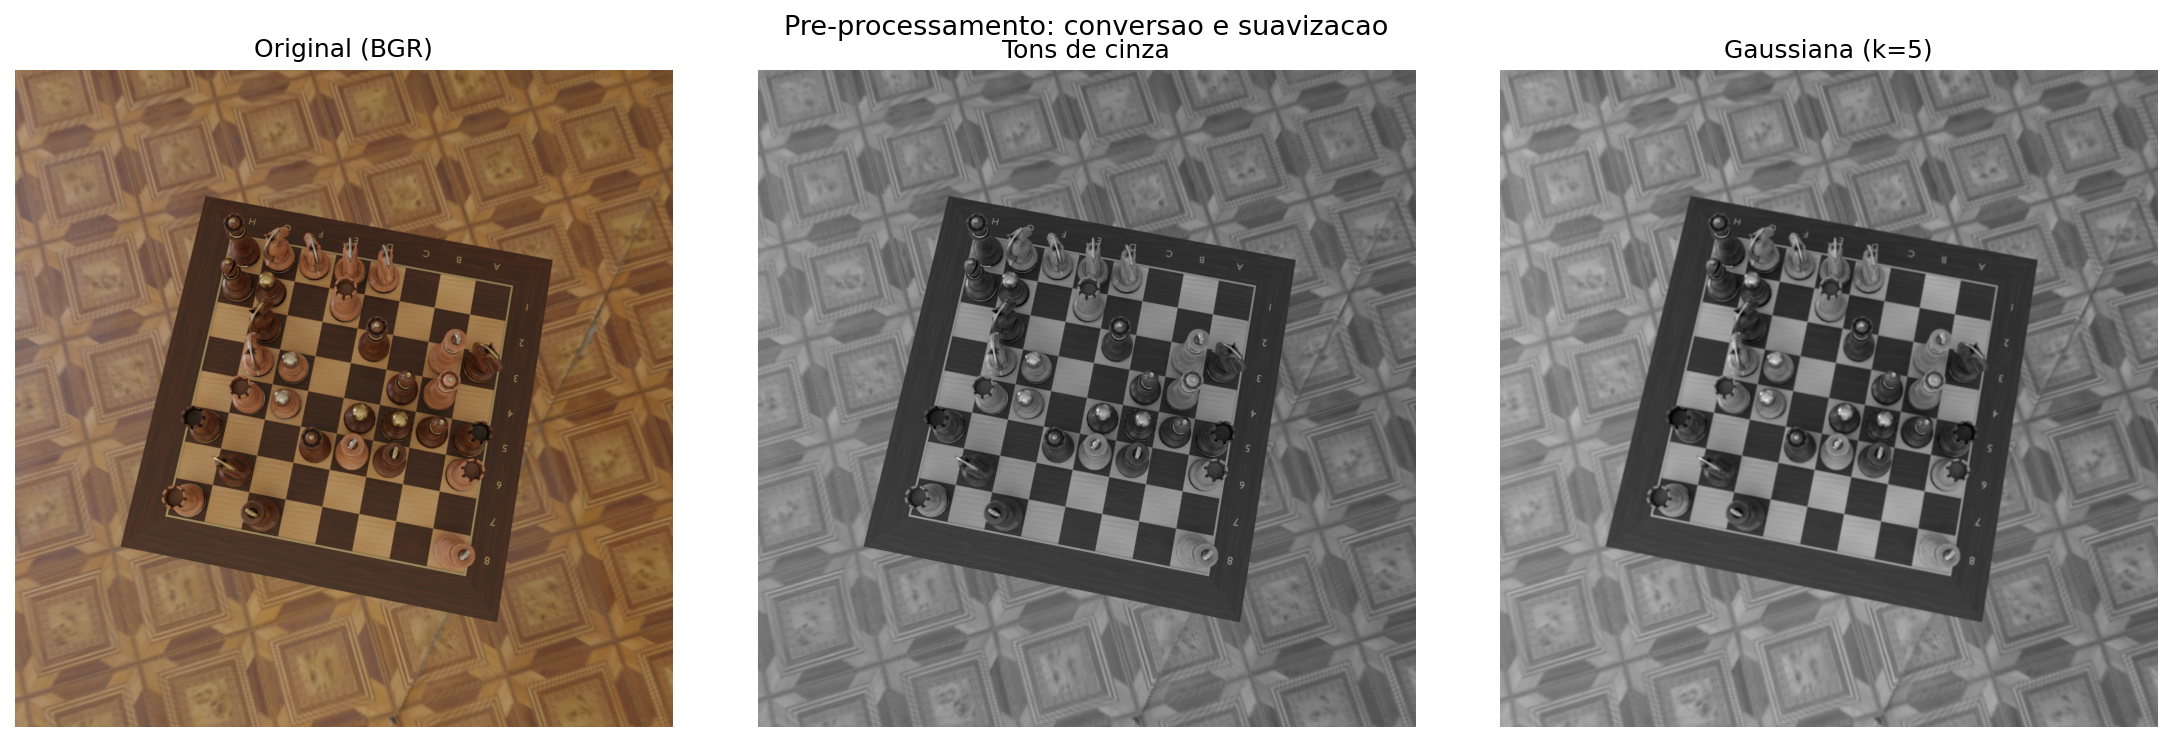
\includegraphics[width=0.75\textwidth]{../../intro/images/03_preprocessing.png}
  \caption{Conversão para tons de cinza e suavização gaussiana.}
\end{figure}

\subsection{Detecção de bordas}

Quatro operadores foram comparados: Roberts (kernel $2\times2$ cruzado, muito sensível a
ruído), Prewitt (kernel $3\times3$, suavização uniforme), Sobel (kernel $3\times3$
ponderado, mais peso no centro) e Canny (pipeline multi-etapa com supressão de
não-máximos e histerese). O Canny foi escolhido para o restante da pipeline por ser o
mais robusto, com limiares $\text{low}=50$, $\text{high}=150$ --- um compromisso entre
sensibilidade excessiva ($30,80$, capta ruído) e conservadorismo ($80,200$, perde bordas
fracas relevantes).

\begin{figure}[H]
  \centering
  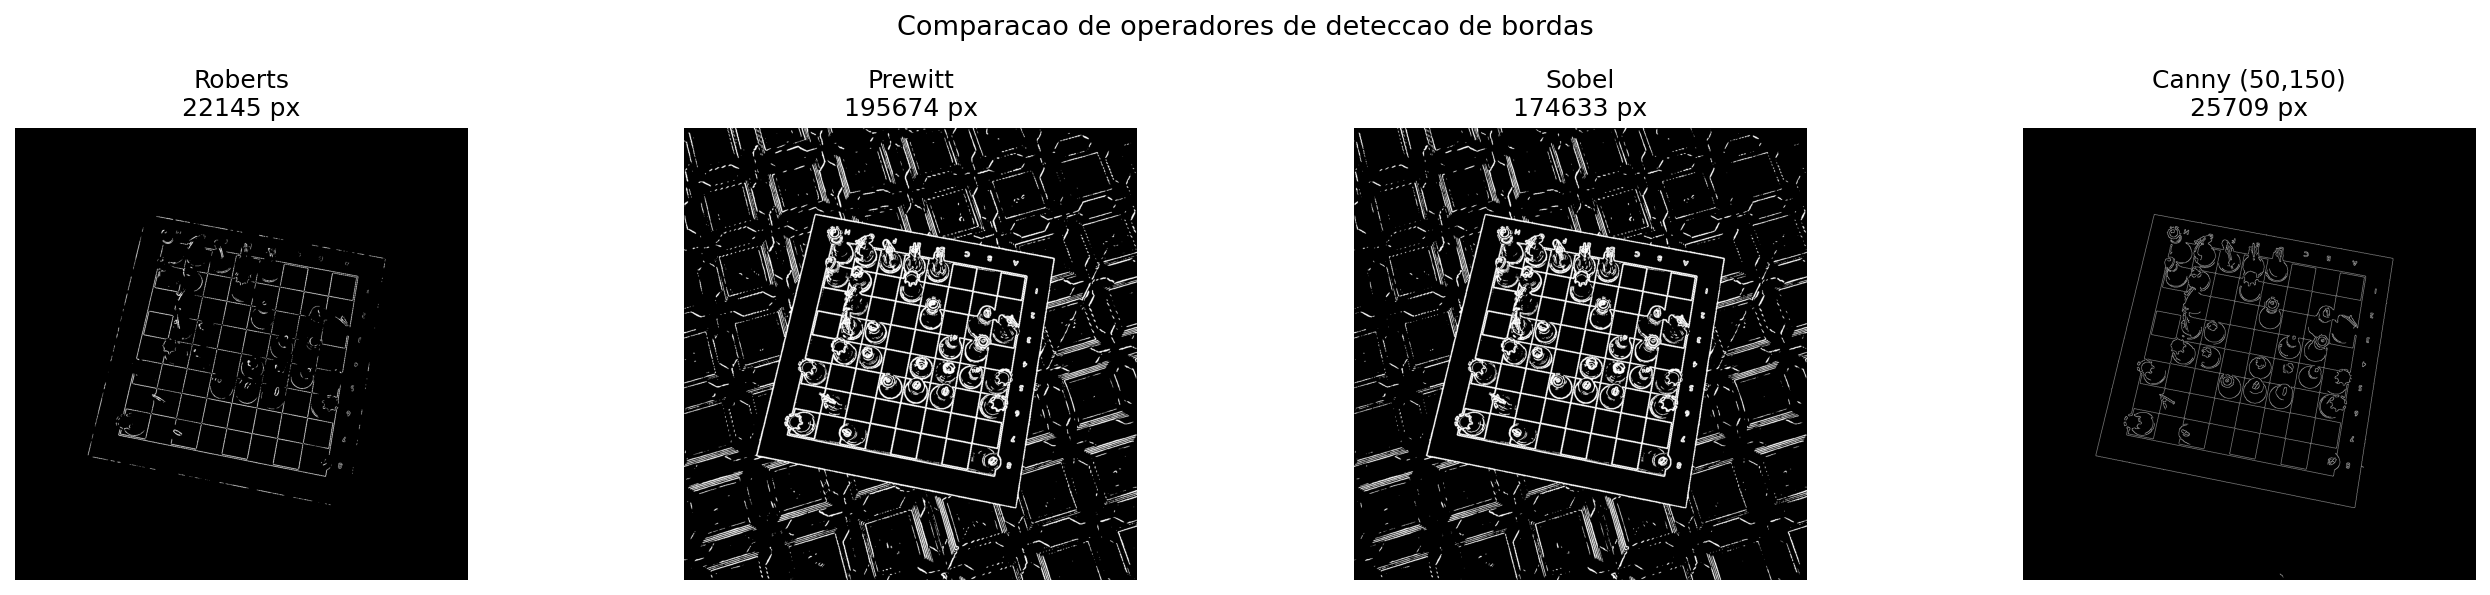
\includegraphics[width=0.85\textwidth]{../../intro/images/04b_edge_operators_comparison.png}
  \caption{Comparação entre operadores de borda Roberts, Prewitt, Sobel e Canny.}
\end{figure}

Operações morfológicas (erosão e dilatação $3\times3$, abertura e fechamento
$5\times5$) são aplicadas sobre a imagem binária de bordas para remover ruído pontual e
conectar segmentos de borda próximos.

\subsection{Detecção de linhas --- Transformada de Hough}

A Transformada de Hough converte o problema de detectar linhas no espaço da imagem em
detectar picos no espaço paramétrico $(\rho, \theta)$: cada pixel de borda vota em todas
as curvas $\rho = x\cos\theta + y\sin\theta$ compatíveis, e picos do acumulador acima de
um limiar indicam linhas reais (\texttt{cv2.HoughLines}, $\rho=1\,\text{px}$,
$\theta=\pi/180\,\text{rad}$, \texttt{threshold} entre 80 e 100).

As linhas detectadas são classificadas em horizontais ($\theta \approx \pi/2$) e
verticais ($\theta \approx 0$). Um algoritmo de janela deslizante seleciona, em cada
direção, as 9 linhas mais igualmente espaçadas, correspondendo às 9 linhas de grade do
tabuleiro $8\times8$. O dataset inclui uma borda de madeira ao redor do grid de jogo; a
última linha horizontal detectada corresponde a essa borda e é descartada --- os cantos
do tabuleiro de jogo são calculados usando a penúltima linha como borda inferior real.

\begin{figure}[H]
  \centering
  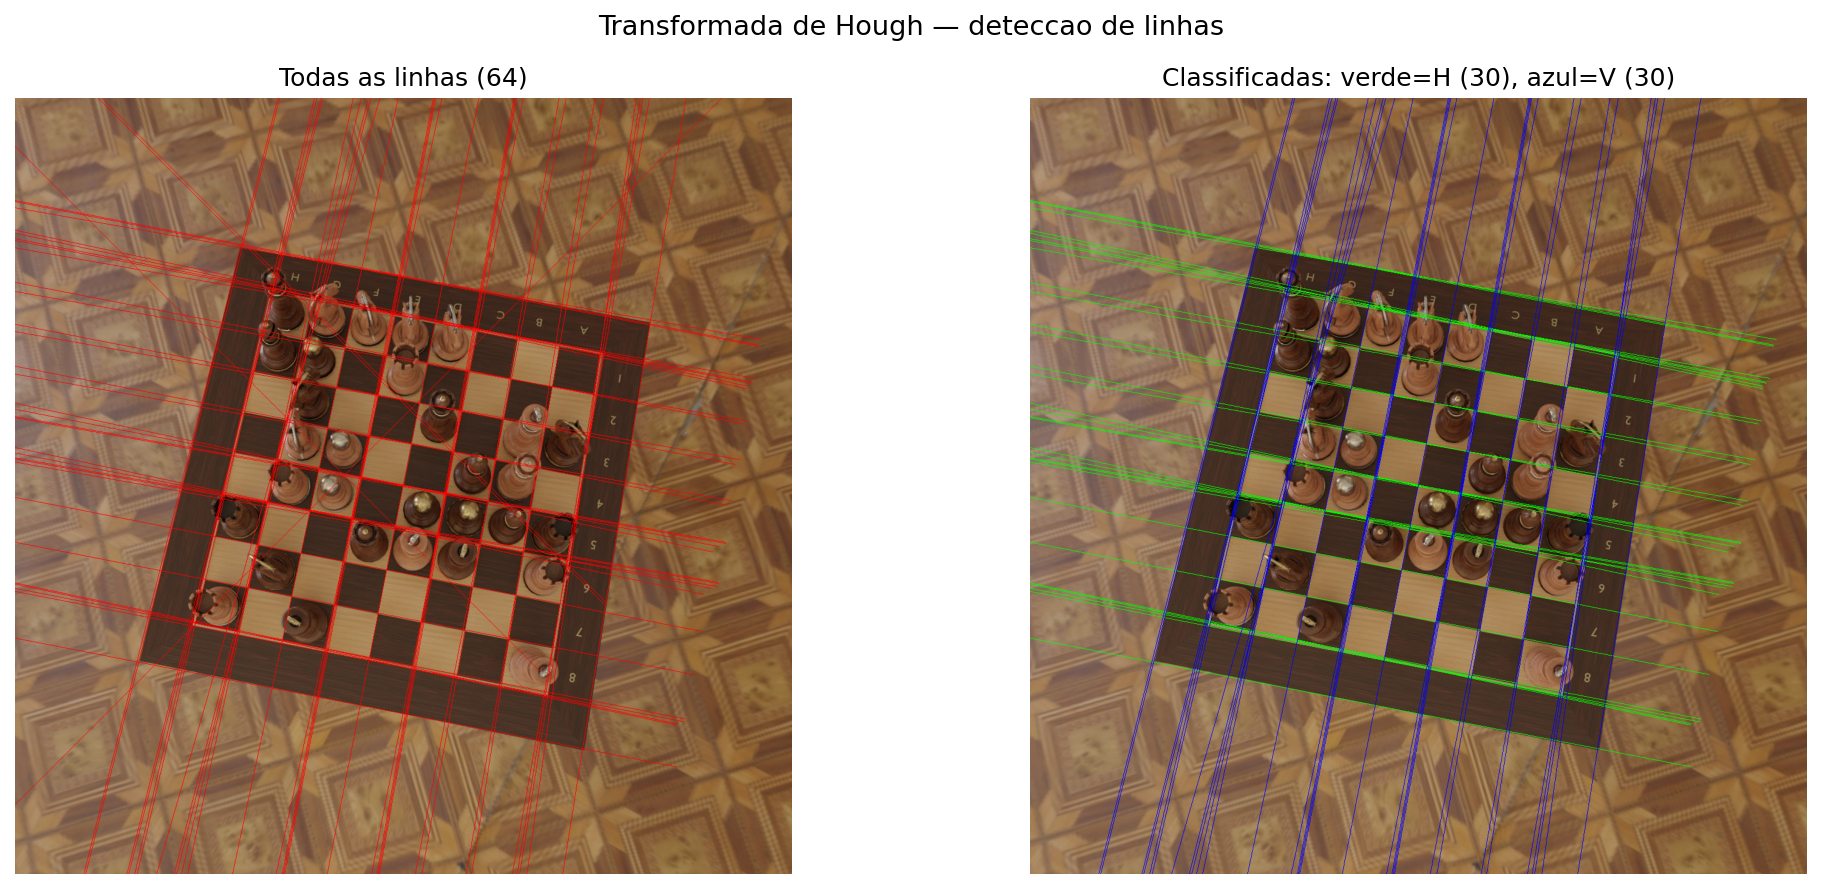
\includegraphics[width=0.7\textwidth]{../../intro/images/05_hough_lines.png}
  \caption{Linhas horizontais (verde) e verticais (azul) detectadas via Hough.}
\end{figure}

\subsection{Correção de perspectiva --- homografia}

Uma homografia (matriz projetiva $3\times3$) mapeia os 4 cantos detectados do tabuleiro
para os cantos de um quadrado de destino de $480\times480$ pixels
(\texttt{cv2.findHomography} + \texttt{cv2.warpPerspective}), produzindo uma vista de
cima onde cada uma das 64 casas ocupa exatamente $60\times60$ pixels. A função de
detecção de cantos (\texttt{detect\_board\_corners\_combined}) executa toda a pipeline
de bordas e Hough sem usar anotações; em caso de falha, os cantos anotados no JSON do
dataset são usados como \textit{fallback}.

Como a câmera fotografa o tabuleiro de ângulos variados, a orientação do mapa de
ocupação resultante pode estar rotacionada em $0\degree$, $90\degree$, $180\degree$ ou
$270\degree$ em relação ao referencial padrão. Quando o \textit{ground truth} está
disponível, a rotação correta é escolhida por busca exaustiva entre as 4 opções
(\texttt{best\_rotation\_vs\_gt}); no cenário totalmente automático, a orientação é
estimada a partir da densidade de bordas por linha/coluna
(\texttt{detect\_board\_rotation}) --- ver discussão da ambiguidade de $180\degree$ na
Seção~\ref{sec:fen-jogadas}.

\begin{figure}[H]
  \centering
  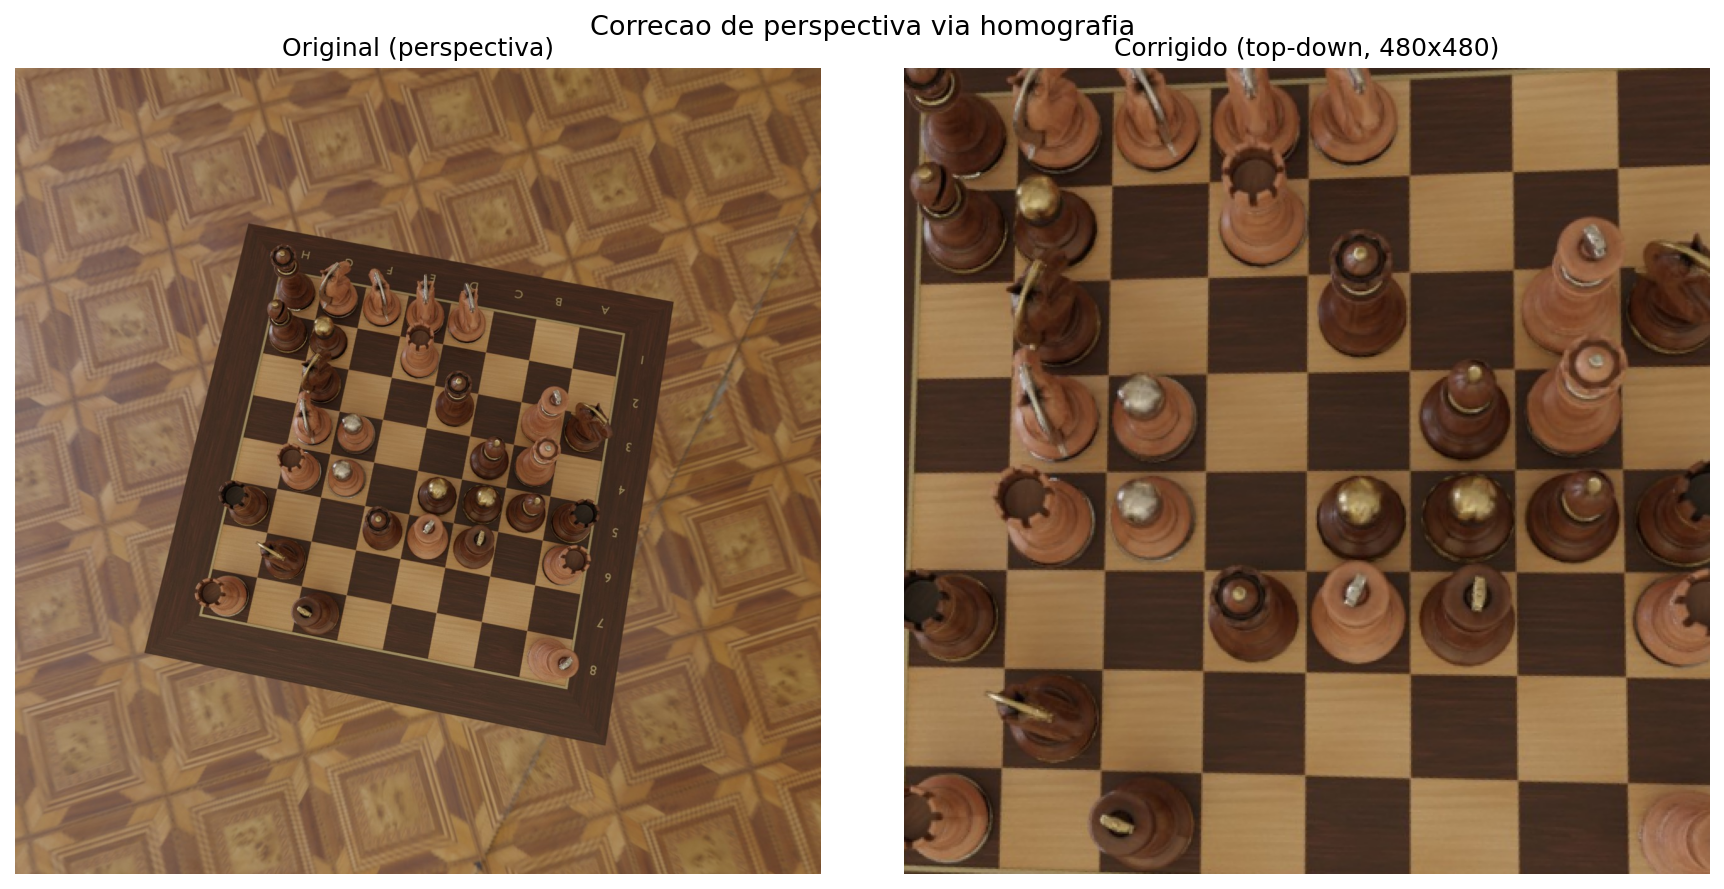
\includegraphics[width=0.6\textwidth]{../../intro/images/07_perspective_correction.png}
  \caption{Correção de perspectiva: da foto em ângulo à vista de cima $480\times480$.}
\end{figure}

\subsection{Segmentação $8\times8$}

Com o tabuleiro retificado, a divisão em 64 casas é um fatiamento uniforme:
$\text{cell}_{r,c} = \text{warped}[r{\cdot}60:(r{+}1){\cdot}60,\; c{\cdot}60:(c{+}1){\cdot}60]$,
produzindo recortes de $60\times60$ pixels indexados de A1 a H8.

\begin{figure}[H]
  \centering
  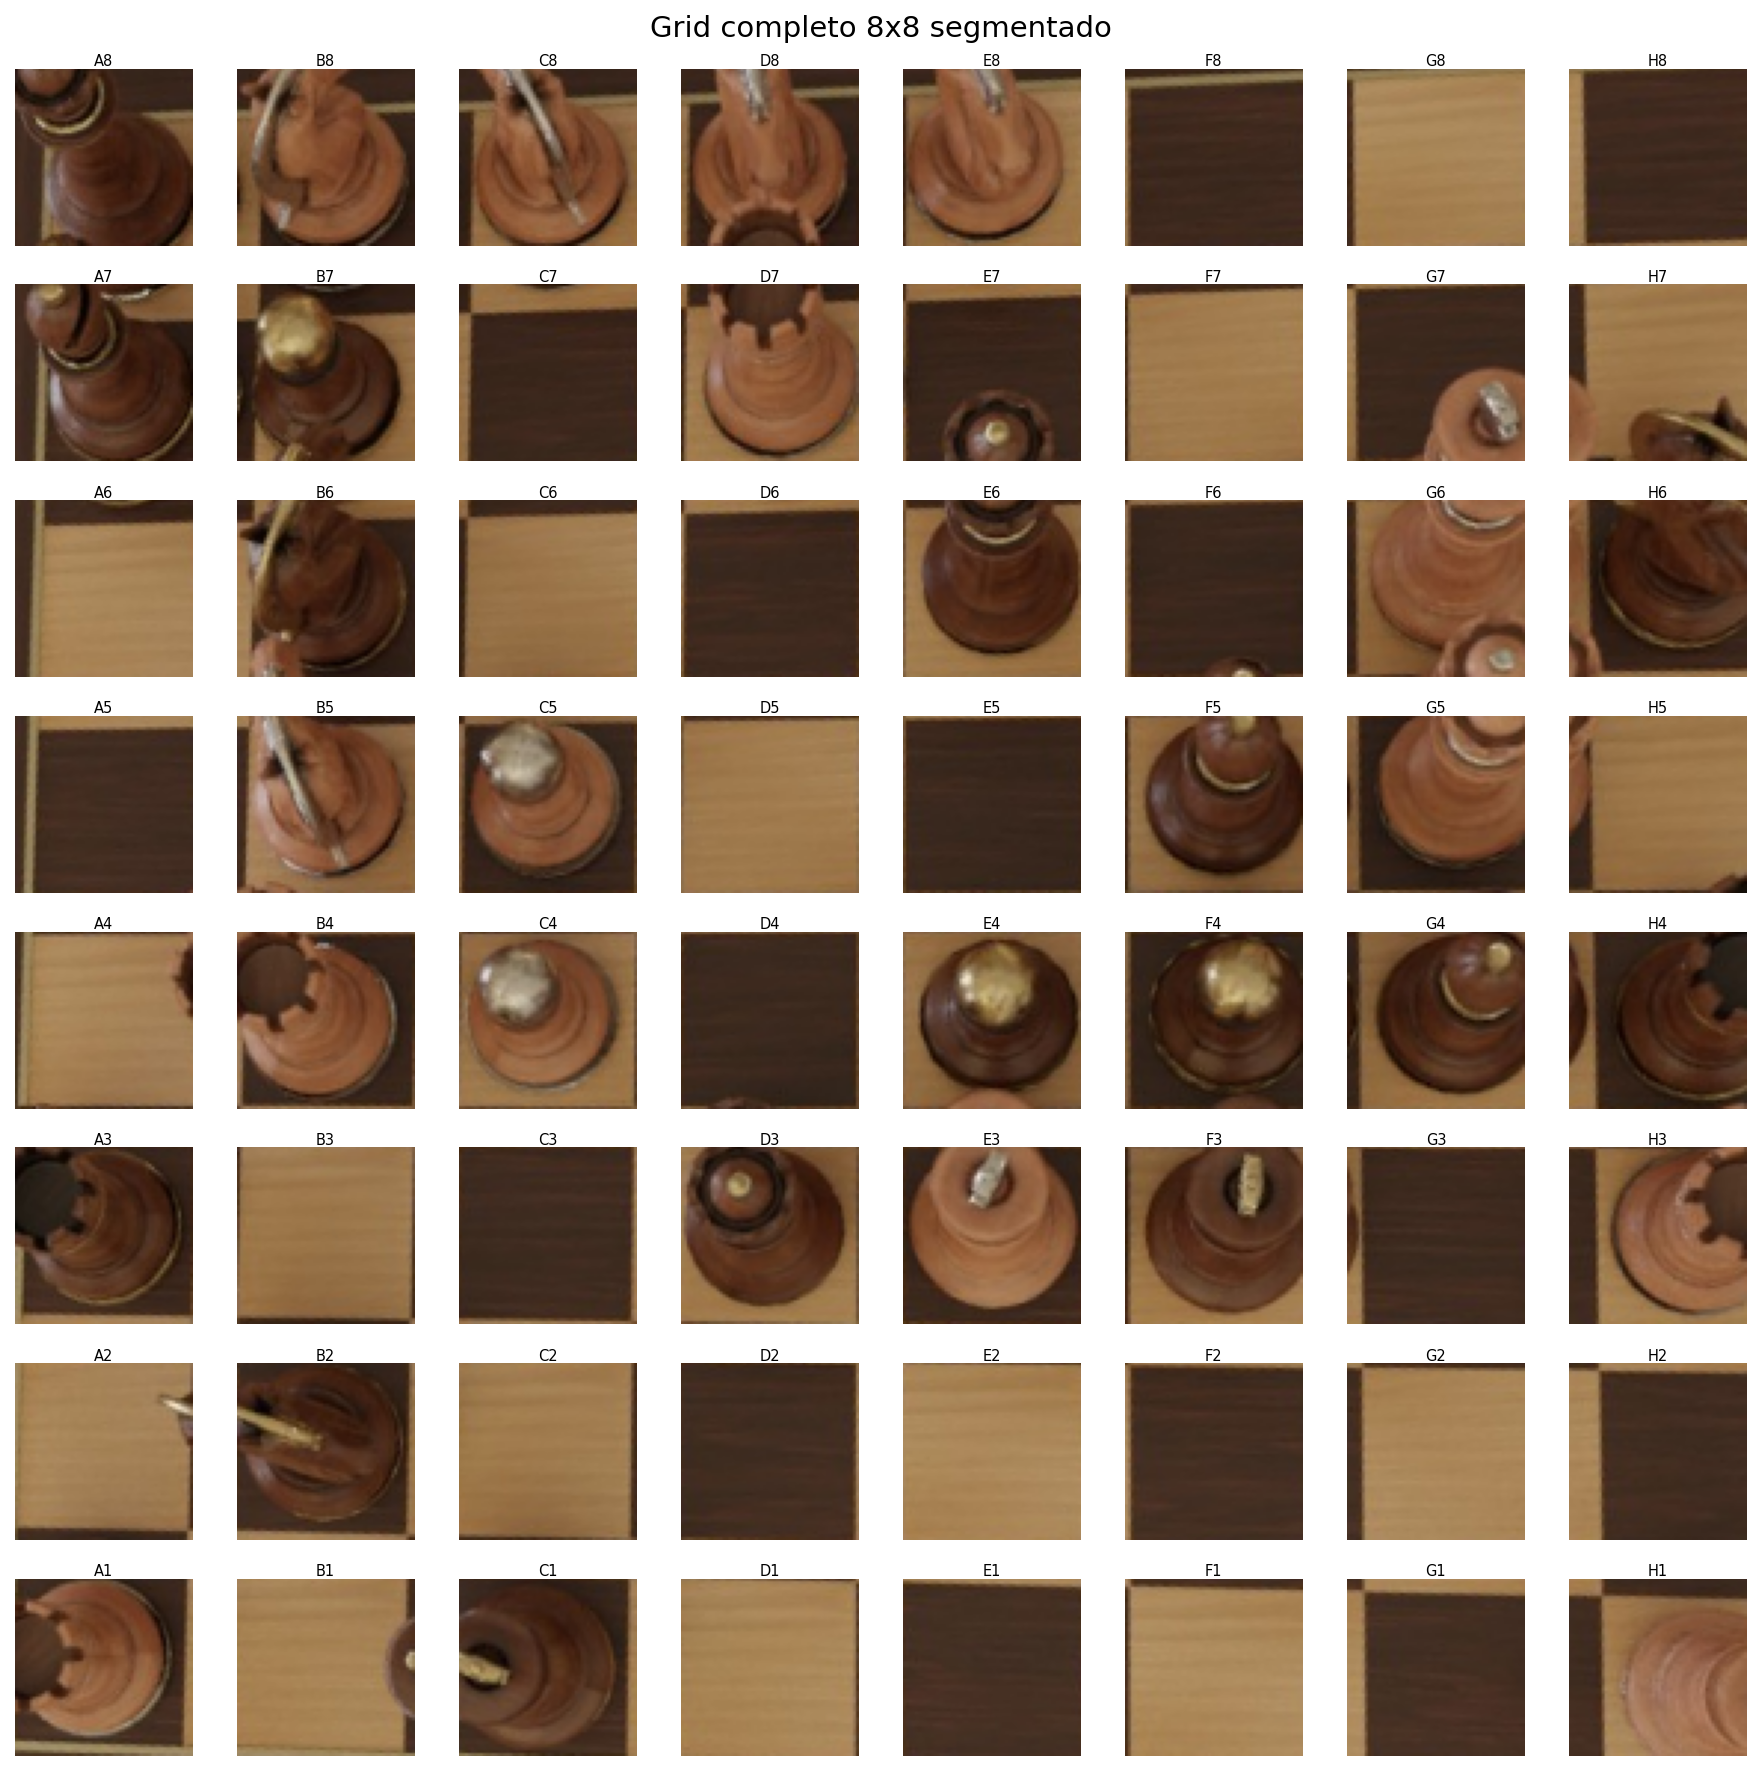
\includegraphics[width=0.55\textwidth]{../../intro/images/08_full_grid.png}
  \caption{Segmentação do tabuleiro retificado em 64 casas individuais.}
\end{figure}

\subsection{Detecção de ocupação}

Para cada casa, quatro descritores clássicos são extraídos e combinados por votação:

\begin{table}[H]
\centering
\caption{Características e limiares do classificador de ocupação por votação.}
\begin{tabular}{@{}llll@{}}
\toprule
Característica & Cálculo & Limiar & Lógica \\
\midrule
Desvio-padrão de intensidade & \texttt{np.std(cell)} & 18 & peças criam variação de brilho \\
Densidade de bordas & \texttt{mean(canny > 0)} & 0,04 & peças geram bordas internas \\
Variância do Laplaciano & \texttt{Laplacian(cell).var()} & 80 & indica textura (peça $\ne$ madeira lisa) \\
Diferença centro-borda & \texttt{mean(centro) - mean(borda)} & 12 & peça ocupa o centro da casa \\
\bottomrule
\end{tabular}
\end{table}

A casa é considerada ocupada quando pelo menos 2 das 4 características ultrapassam seu
limiar (\textit{votos} $\geq 2$). Com material uniforme (madeira sobre madeira), nenhuma
característica isolada é confiável o suficiente; a combinação por maioria simples reduz
falsos positivos e negativos em relação a qualquer característica isolada.

\begin{figure}[H]
  \centering
  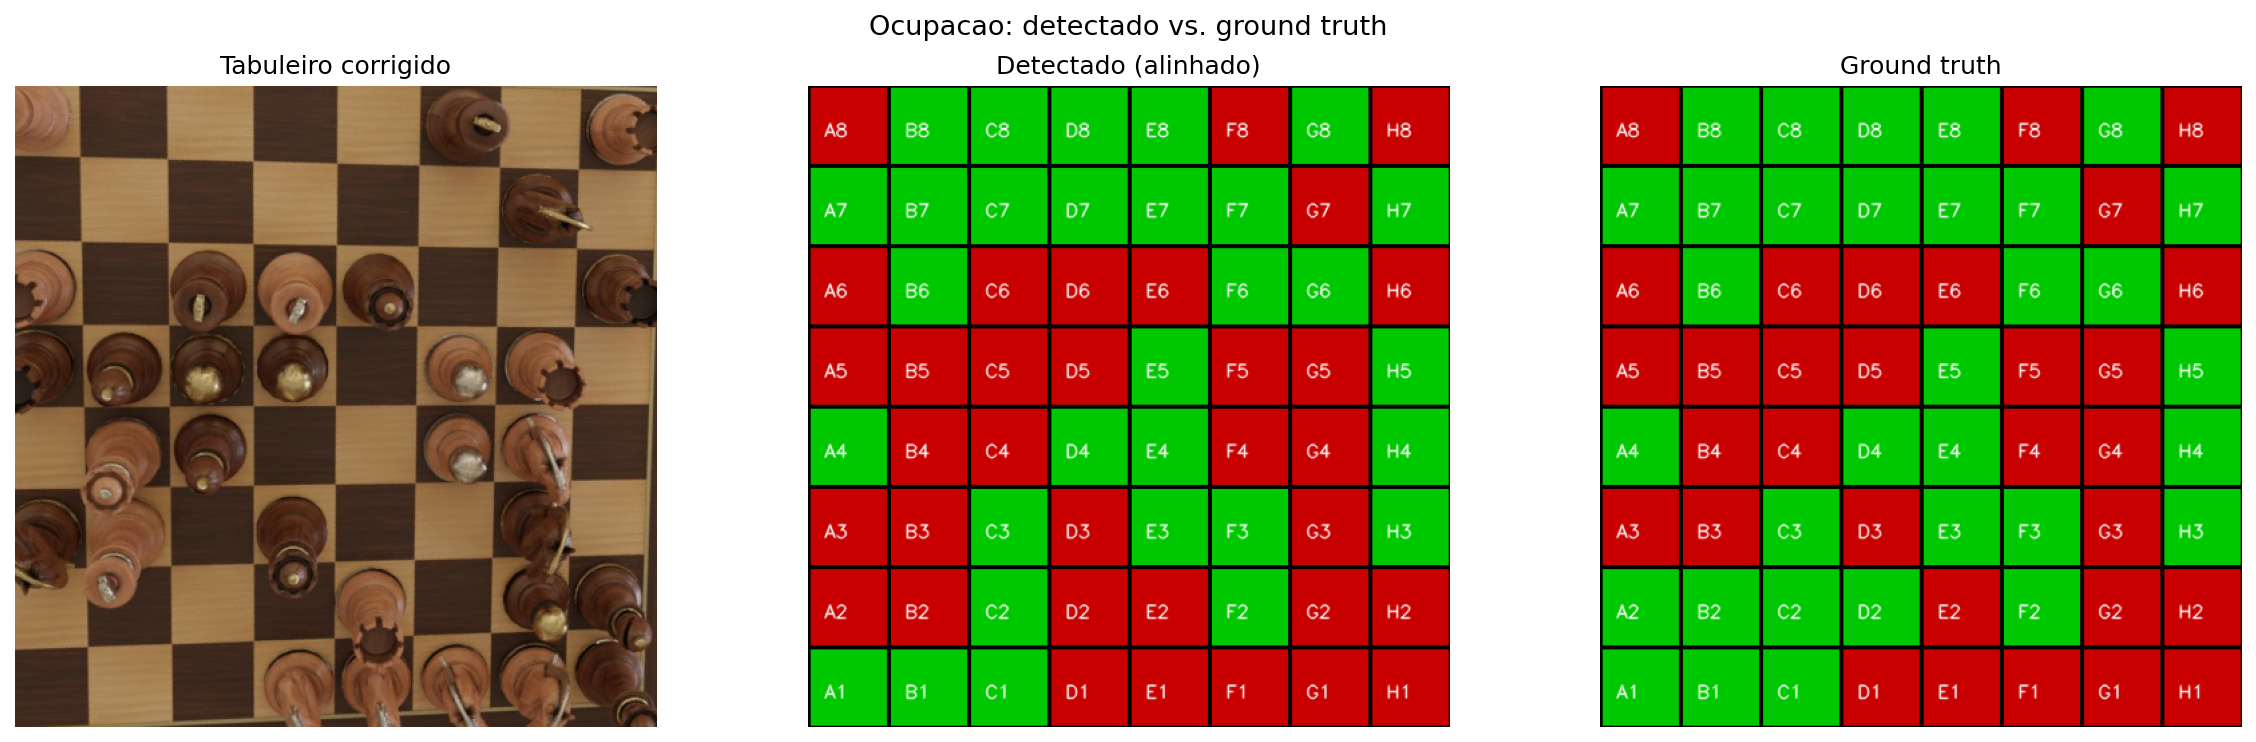
\includegraphics[width=0.7\textwidth]{../../intro/images/10_occupancy_comparison.png}
  \caption{Ocupação detectada (vermelho = ocupada, verde = vazia) comparada ao gabarito.}
\end{figure}

\subsection{Classificação de cor}

A cor de cada peça (clara ou escura) é decidida pelo canal V (\textit{value}, brilho) do
espaço HSV: \texttt{mean\_v = np.mean(hsv[:,:,2])}; peças com \texttt{mean\_v} acima de
um limiar fixo são classificadas como claras, abaixo como escuras. Peças claras
(\textit{boxwood}) têm maior brilho médio que peças escuras (\textit{ebony}), o que
torna essa distinção robusta na maior parte das imagens --- exceto em casos de sombra
projetada ou peça escura sobre casa escura, onde o limiar fixo falha (ver
Seção~\ref{sec:resultados}).

\begin{figure}[H]
  \centering
  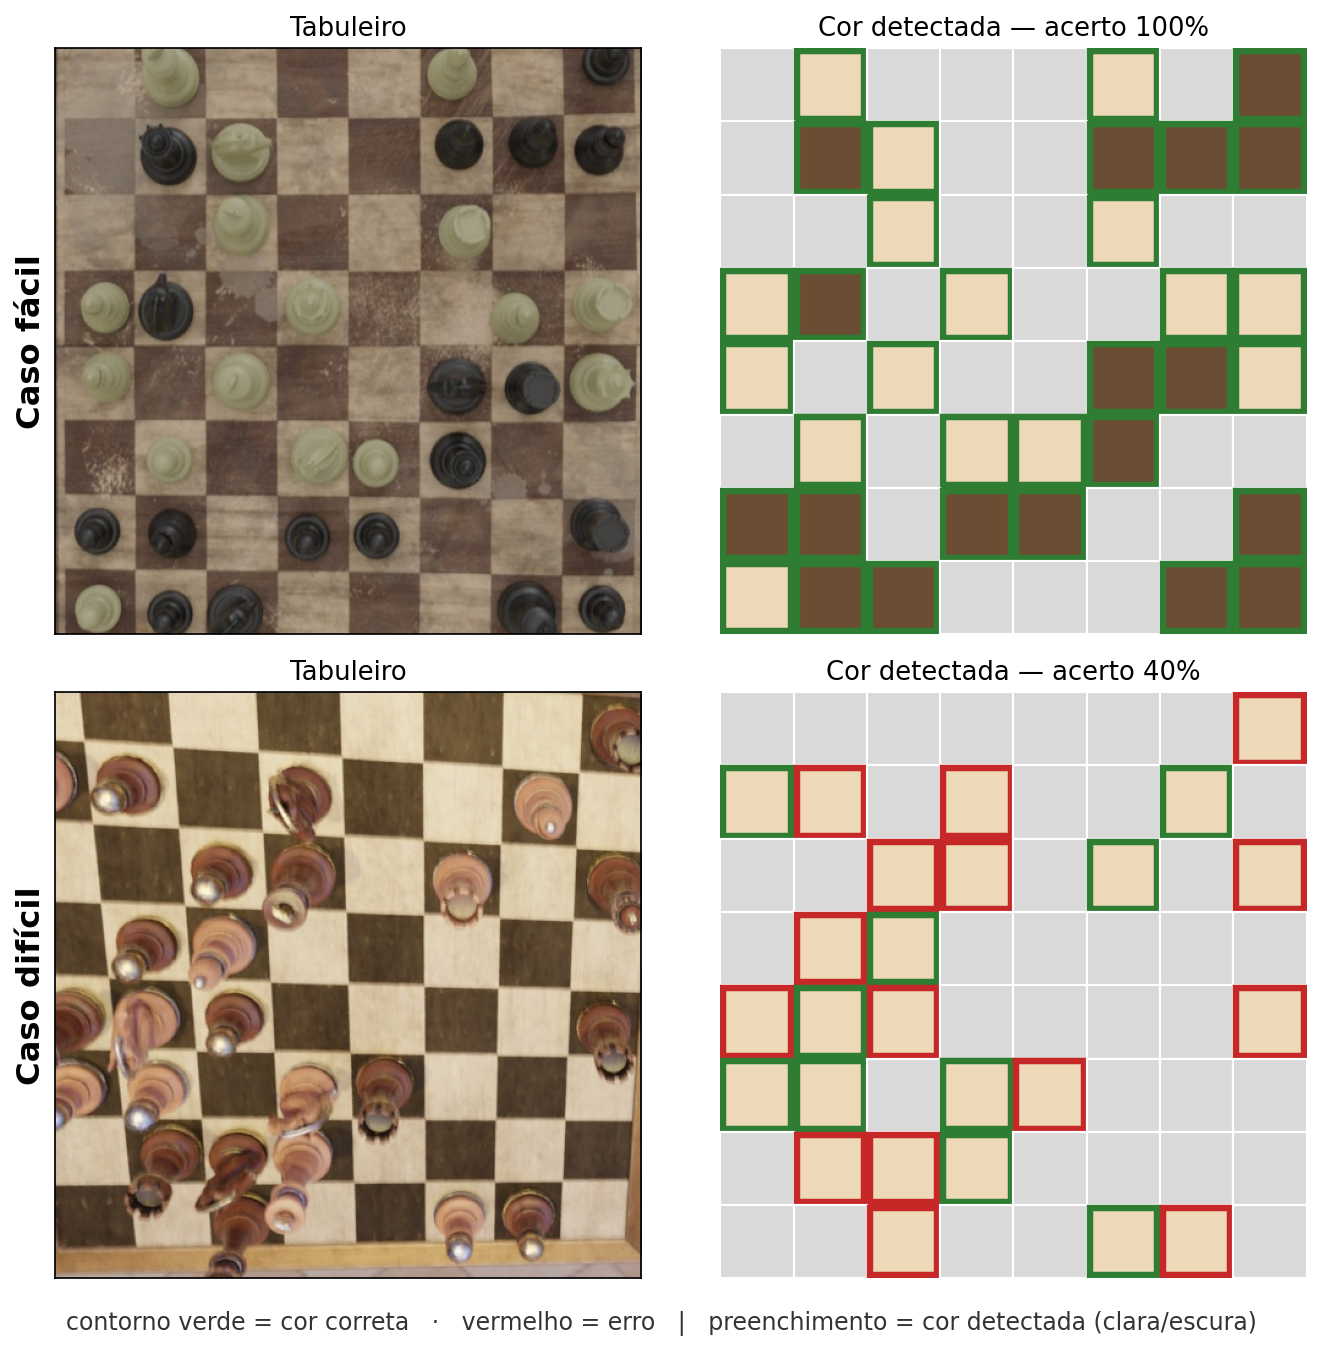
\includegraphics[width=0.6\textwidth]{../../andamento/images/11b_color_cases.png}
  \caption{Casos fáceis e difíceis de classificação de cor por limiar HSV.}
\end{figure}

\section{Classificação do Tipo de Peça: \textit{Transfer Learning} com ResNet-34}
\label{sec:deep-learning}

\subsection{Motivação}

Abordagens clássicas de reconhecimento de forma (\textit{template matching},
momentos de Hu, contornos, HOG) foram descartadas para esta etapa após avaliação
preliminar, por três razões: (i) baixo contraste peça-tabuleiro, ambos em madeira; (ii)
deformação de perspectiva da silhueta das peças, que varia com o ângulo de câmera; (iii)
silhuetas intrinsecamente parecidas entre classes (peão $\times$ bispo, torre $\times$
dama em determinados ângulos). Optou-se por \textit{transfer learning} com uma rede
convolucional pré-treinada, mantendo clássico tudo o que vem antes (Seção
\ref{sec:metodologia}).

\subsection{Arquitetura}

A \textbf{ResNet-34} \cite{resnet}, pré-treinada no ImageNet \cite{imagenet}, tem sua
camada final substituída por uma camada linear de 12 saídas (uma por classe de
peça$\times$cor): \texttt{pawn\_w}, \texttt{pawn\_b}, \texttt{rook\_w},
\texttt{rook\_b}, \texttt{knight\_w}, \texttt{knight\_b}, \texttt{bishop\_w},
\texttt{bishop\_b}, \texttt{queen\_w}, \texttt{queen\_b}, \texttt{king\_w},
\texttt{king\_b}. A escolha da ResNet-34 (34 camadas convolucionais, cerca de 21
milhões de parâmetros) equilibra capacidade de representação e risco de
\textit{overfitting} dado o volume de dados de treino disponível (\textasciitilde62\,000
células).

\subsection{Construção do dataset de treinamento}

Para cada imagem do dataset original, o tabuleiro é retificado usando os cantos do
gabarito, a orientação é determinada automaticamente por densidade de bordas, e cada
casa ocupada é recortada e salva em \texttt{outputs/piece\_cells/\{classe\}/}, rotulada
pelo tipo e cor da peça segundo o gabarito. O volume resultante é de
aproximadamente $1\,944$ imagens $\times$ \textasciitilde32 peças $\approx$
\textbf{62\,000} recortes de $64\times64$ pixels (redimensionados para $224\times224$ no
\textit{dataloader}), com classes aproximadamente balanceadas (peões ligeiramente mais
frequentes, cerca de 3$\times$ mais que reis/rainhas). O conjunto é dividido em 80\% de
treino e 20\% de validação, estratificado por classe.

\subsection{Treinamento em duas fases}

\subsubsection{Fase 1 --- \textit{Transfer learning} (cabeça congelada)}

O corpo da rede (\texttt{backbone}) é congelado e apenas a nova camada classificadora é
treinada, por 10 épocas, com otimizador Adam ($\text{lr}=10^{-3}$), \textit{cross-entropy}
e \textit{scheduler} \texttt{CosineAnnealingLR}. Essa fase é segura por construção: como
o restante da rede está congelado, não há risco de destruir as características herdadas
do ImageNet enquanto a cabeça, ainda aleatória, se ajusta.

\subsubsection{Fase 2 --- \textit{Fine-tuning} (rede inteira)}

Toda a rede é descongelada e re-treinada por 15 épocas com taxas de aprendizado
discriminativas por grupo de camadas --- menores nas camadas iniciais, que já contêm
características genéricas úteis (bordas, texturas), e maiores nas camadas finais e na
cabeça:

\begin{table}[H]
\centering
\caption{Hiperparâmetros da Fase 2 (\textit{fine-tuning}).}
\begin{tabular}{@{}ll@{}}
\toprule
Hiperparâmetro & Valor / justificativa \\
\midrule
LR base (cabeça / \texttt{layer4}) & $3\times10^{-5}$ --- muito menor que a Fase 1, preserva features ImageNet \\
Decaimento por camada & $\times 0{,}3$ por bloco anterior --- camadas iniciais precisam de ajuste mínimo \\
Otimizador & AdamW, \texttt{weight\_decay}=$10^{-4}$ (regularização) \\
\textit{Label smoothing} & 0,1 --- ajuda classes raras (rei, dama) \\
\textit{Warmup} & 2 épocas lineares --- evita destruir features no início do \textit{fine-tuning} \\
\textit{Gradient clipping} & norma máxima 1,0 --- estabiliza treino com LR discriminativo \\
Precisão mista (AMP) & \texttt{GradScaler} --- acelera treino em GPU \\
\bottomrule
\end{tabular}
\end{table}

O aumento de dados (\textit{data augmentation}) aplicado a cada época inclui
espelhamento horizontal e vertical, rotação aleatória de até $15\degree$ e variação de
brilho/contraste/saturação, seguido de redimensionamento para $224\times224$ e
normalização no padrão ImageNet. O treinamento é feito em GPU (CUDA), em lotes de 64
imagens.

\subsection{Impacto do \textit{fine-tuning}}

O ganho da Fase 2 é substancial e concentrado nas classes raras: com apenas 1 época de
\textit{fine-tuning}, o F1 global era de 53,2\%; após as 15 épocas completas com as
práticas acima, o F1 sobe para \textbf{91,0\%}. O impacto é mais visível nas classes
menos frequentes: \texttt{king\_b} sai de 14,2\% para 84,5\% de acurácia, e
\texttt{queen\_w} de 27,7\% para 90,8\%. Os resultados quantitativos completos, por
classe, estão na Seção~\ref{sec:resultados}.

\section{Reconstrução de FEN e Detecção de Jogadas}
\label{sec:fen-jogadas}

Com um \texttt{piece\_map} completo (casa $\to$ tipo e cor da peça), obtido combinando a
ocupação clássica, a cor clássica e o tipo previsto pela ResNet-34, a posição pode ser
serializada em \textbf{FEN} (\textit{Forsyth-Edwards Notation}), a notação padrão para
posições de xadrez.

\subsection{FEN completa --- seis campos}

A função \texttt{board\_to\_fen} produz uma FEN \textbf{completa}: o campo de
posicionamento de peças é lido diretamente do tabuleiro (fileira 8 $\to$ 1, maiúsculas
para peças brancas, casas vazias colapsadas em contagens), enquanto os outros cinco
campos --- lado a mover, direitos de roque, alvo de \textit{en passant}, contador de
meio-lances e número da jogada --- são fornecidos explicitamente e validados, pois não
podem ser inferidos a partir de uma única fotografia estática. A função
\texttt{castling\_rights\_from\_position} produz uma estimativa de melhor esforço dos
direitos de roque a partir de onde reis e torres estão posicionados (rei e torre nas
casas de origem $\Rightarrow$ direito de roque presumido).

\subsection{Ambiguidade de orientação de $180\degree$}

Ao ler uma imagem de forma totalmente automática (sem gabarito), a orientação do
tabuleiro é obtida a partir da densidade de bordas por linha/coluna
(\texttt{detect\_board\_rotation}). Essa heurística fixa corretamente o \textbf{eixo} do
tabuleiro (0\% de erro de eixo medido sobre 60 imagens), mas não resolve a ambiguidade de
$180\degree$: como as cores das casas de um tabuleiro de xadrez são simétricas sob
rotação de $180\degree$, não há, a partir de uma única imagem, informação suficiente
para decidir entre as duas orientações --- cerca de \textbf{42\%} dos tabuleiros ficam
efetivamente invertidos nessa leitura totalmente automática.

Isso não é tratado como um defeito a ser corrigido, mas como um \textbf{limite
intrínseco de uma imagem única}, documentado explicitamente: a função
\texttt{rotate\_piece\_map\_180} gera o mapa de peças da orientação alternativa, e o
sistema reporta \textbf{as duas FENs candidatas} --- o tabuleiro real é necessariamente
uma delas. Resolver a ambiguidade remanescente exigiria informação externa à imagem
(OCR dos rótulos de fileira/coluna do próprio tabuleiro físico, ou contexto de uma
partida em andamento), nenhuma das quais confiável neste dataset de imagens isoladas.

\subsection{Detecção de jogadas}

A comparação temporal entre dois mapas de ocupação booleanos identifica as casas que
mudaram de estado:

\begin{lstlisting}[language=Python]
def detect_moves(occ_a, occ_b):
    emptied  = occ_a & ~occ_b   # estava ocupada, agora vazia
    occupied = ~occ_a & occ_b   # estava vazia, agora ocupada
    return list(...)            # lista de (linha, coluna, tipo_de_mudanca)
\end{lstlisting}

Para uma jogada simples, espera-se exatamente 1 casa esvaziada e 1 casa ocupada; uma
captura resulta em 1 casa esvaziada e 0 ou 1 casa ocupada, dependendo de qual lado
capturou. A função \texttt{classify\_move} vai além do diff de ocupação: comparando dois
\texttt{piece\_map}s completos (antes/depois), ela infere o lance em notação UCI e uma
descrição textual, cobrindo os casos especiais do xadrez:

\begin{itemize}[nosep]
  \item \textbf{Lance simples} (ex.: \texttt{1.e4});
  \item \textbf{Captura} (ex.: \texttt{exd5});
  \item \textbf{Roque}, curto ou longo (ex.: \texttt{O-O}) --- identificado pelo padrão
        característico de movimentação simultânea de rei e torre;
  \item \textbf{\textit{En passant}} --- identificado quando um peão captura
        lateralmente sem que a casa capturada coincida com a casa de destino;
  \item \textbf{Promoção} (ex.: \texttt{e8=Q}) --- identificada quando um peão chega à
        última fileira e a peça na casa de destino muda de tipo.
\end{itemize}

Como o dataset não contém sequências de jogo reais (cada imagem é uma posição
independente), a lógica de \texttt{classify\_move} foi validada com posições
\textbf{controladas} --- montadas manualmente para cobrir cada caso especial --- e,
adicionalmente, aplicada a pares de imagens não relacionadas do dataset apenas para
demonstrar o comportamento da função (sem uma jogada real de referência para comparar).

\begin{figure}[H]
  \centering
  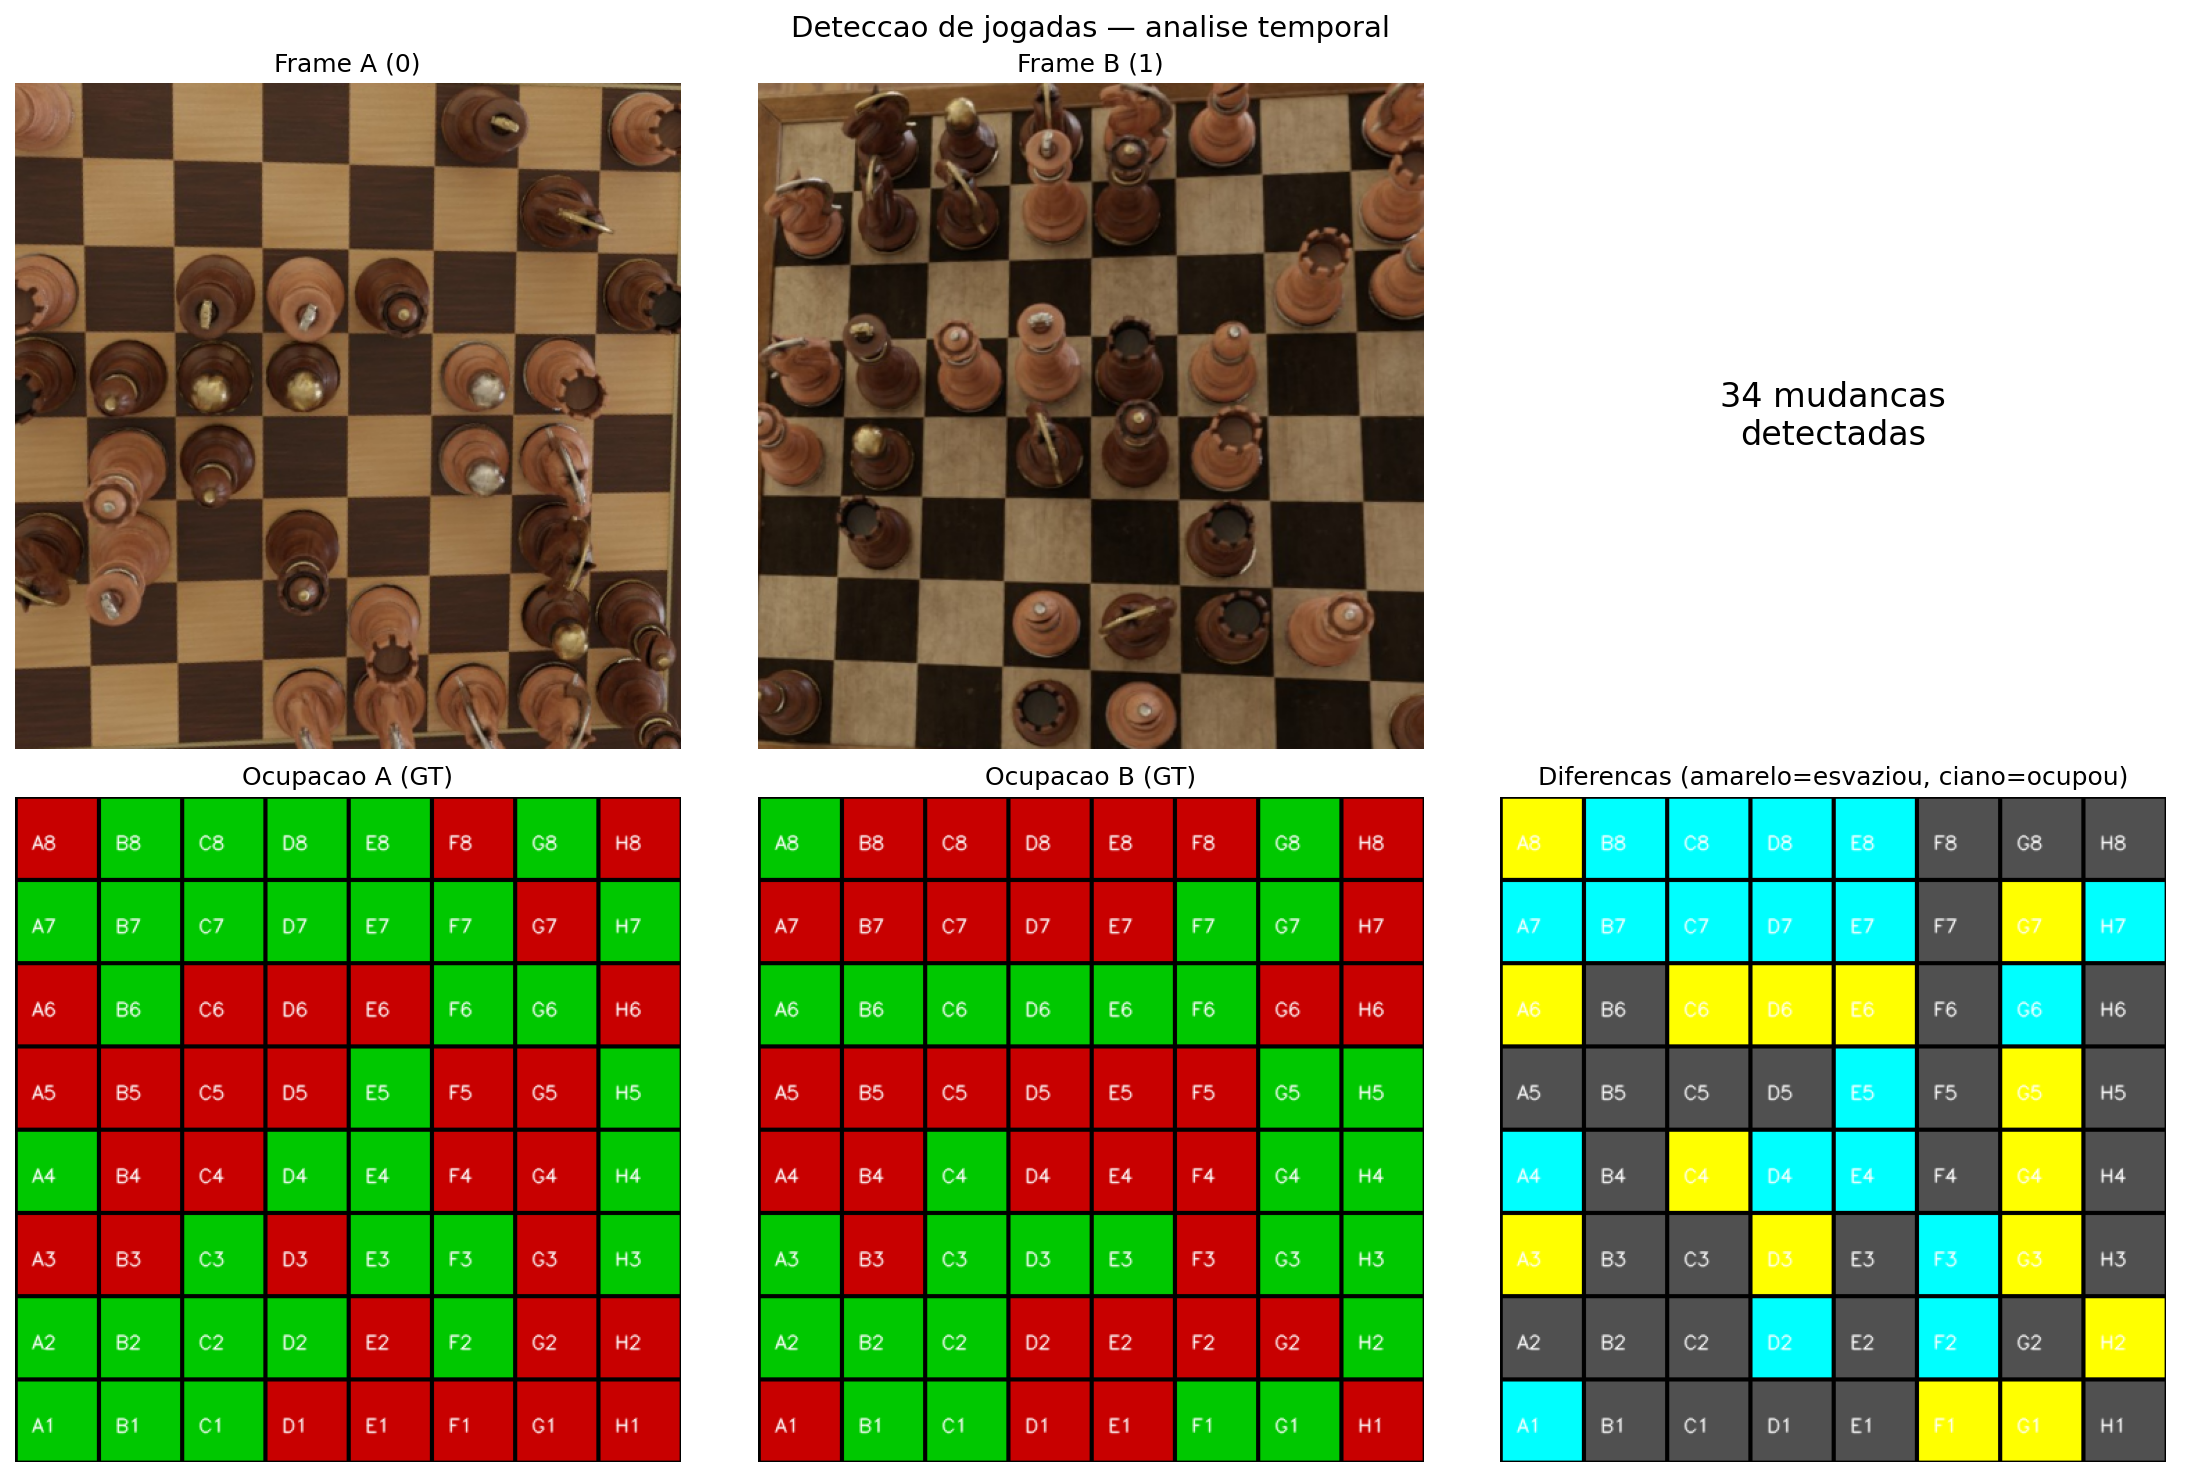
\includegraphics[width=0.85\textwidth]{../../intro/images/12_move_detection.png}
  \caption{Comparação temporal de dois mapas de ocupação: casas esvaziadas (amarelo) e
    ocupadas (ciano).}
\end{figure}

\section{Resultados}
\label{sec:resultados}

Todas as métricas de ponta a ponta e orientação foram reverificadas com o script
reprodutível \texttt{scripts/eval\_metrics.py} (seed fixa, $N=60$ imagens amostradas
aleatoriamente do dataset). Métricas do classificador de tipo de peça e cor foram
avaliadas isolando o classificador da pipeline clássica, ou seja, fornecendo a ocupação
do gabarito (GT) como entrada --- isso evita que erros de ocupação/cantos se propaguem
para a avaliação do classificador de tipo.

\subsection{Detecção de ocupação (pipeline clássica, ponta a ponta)}

\begin{table}[H]
\centering
\caption{Ocupação --- 60 imagens, cantos detectados automaticamente (Hough).}
\begin{tabular}{@{}lrrrr@{}}
\toprule
Métrica & Média & Mediana & Mín. & Máx. \\
\midrule
Acurácia & 64,5\% & 59,4\% & 34,4\% & 98,4\% \\
Precisão & 59,8\% & 58,8\% & 0\% & 100\% \\
Recall   & \textbf{70,2\%} & 79,6\% & 0\% & 100\% \\
F1       & 62,7\% & 66,7\% & 0\% & 98,4\% \\
\bottomrule
\end{tabular}
\end{table}

Com \textbf{cantos do gabarito} (isolando o erro de detecção de cantos do restante da
pipeline), o F1 de ocupação sobe para \textbf{86,3\%} --- confirmando que o gargalo
principal do sistema é a detecção automática dos 4 cantos do tabuleiro, e não a votação
de características de ocupação em si. O recall consistentemente maior que a precisão
indica que o pipeline tende a \textbf{superestimar} a ocupação (marcar casas vazias como
ocupadas) devido ao baixo contraste madeira-sobre-madeira, mais do que a perder peças
existentes.

\subsection{Classificação de cor}

Avaliada com cantos do gabarito sobre 200 imagens, a classificação de cor por limiar
fixo do canal V (HSV) atinge \textbf{82,5\%} de acerto geral. Cerca de 38\% das imagens
são ``fáceis'' (acerto $\geq$ 90\%, bom contraste peça-fundo); 18\% são ``difíceis''
(acerto $<$ 70\%), tipicamente por sombra projetada ou peça escura sobre casa escura, onde
o limiar fixo de brilho falha.

\subsection{Classificação de tipo de peça (ResNet-34)}

Avaliada em 50 imagens com ocupação do gabarito (isola o classificador do restante da
pipeline; FN = FP = 0 por construção, já que a ocupação é fornecida):

\begin{table}[H]
\centering
\caption{Classificador de tipo de peça --- métricas globais.}
\begin{tabular}{@{}lr@{}}
\toprule
Métrica & Valor \\
\midrule
Precisão & 91,0\% \\
Recall   & 91,0\% \\
F1-score & \textbf{91,0\%} \\
Peças corretas (tipo + posição) & 1\,412 \\
Tipo errado (posição certa)     & 140 \\
\bottomrule
\end{tabular}
\end{table}

\begin{table}[H]
\centering
\caption{Acurácia por classe de peça.}
\begin{tabular}{@{}lrl@{}}
\toprule
Classe & Acurácia & Observação \\
\midrule
knight\_b & \textbf{96,4\%} & silhueta do cavalo é distintiva \\
pawn\_b   & 96,3\% & classe mais representada \\
knight\_w & 95,9\% & --- \\
pawn\_w   & 93,8\% & --- \\
queen\_w  & 90,8\% & melhorou de 27,7\% para 90,8\% com \textit{fine-tuning} \\
rook\_w   & 90,1\% & --- \\
rook\_b   & 89,2\% & --- \\
king\_w   & 89,7\% & --- \\
bishop\_w & 87,6\% & --- \\
bishop\_b & 88,2\% & --- \\
queen\_b  & 87,8\% & --- \\
king\_b   & \textbf{84,5\%} & classe mais difícil; efeito residual do desbalanceamento \\
\bottomrule
\end{tabular}
\end{table}

Quando avaliado conjuntamente com a classificação de cor (tipo + cor, ocupação do
gabarito, $N=60$), o acerto é de \textbf{93,0\%}, consistente com o F1 de 91\% medido
isoladamente para o tipo.

\begin{figure}[H]
  \centering
  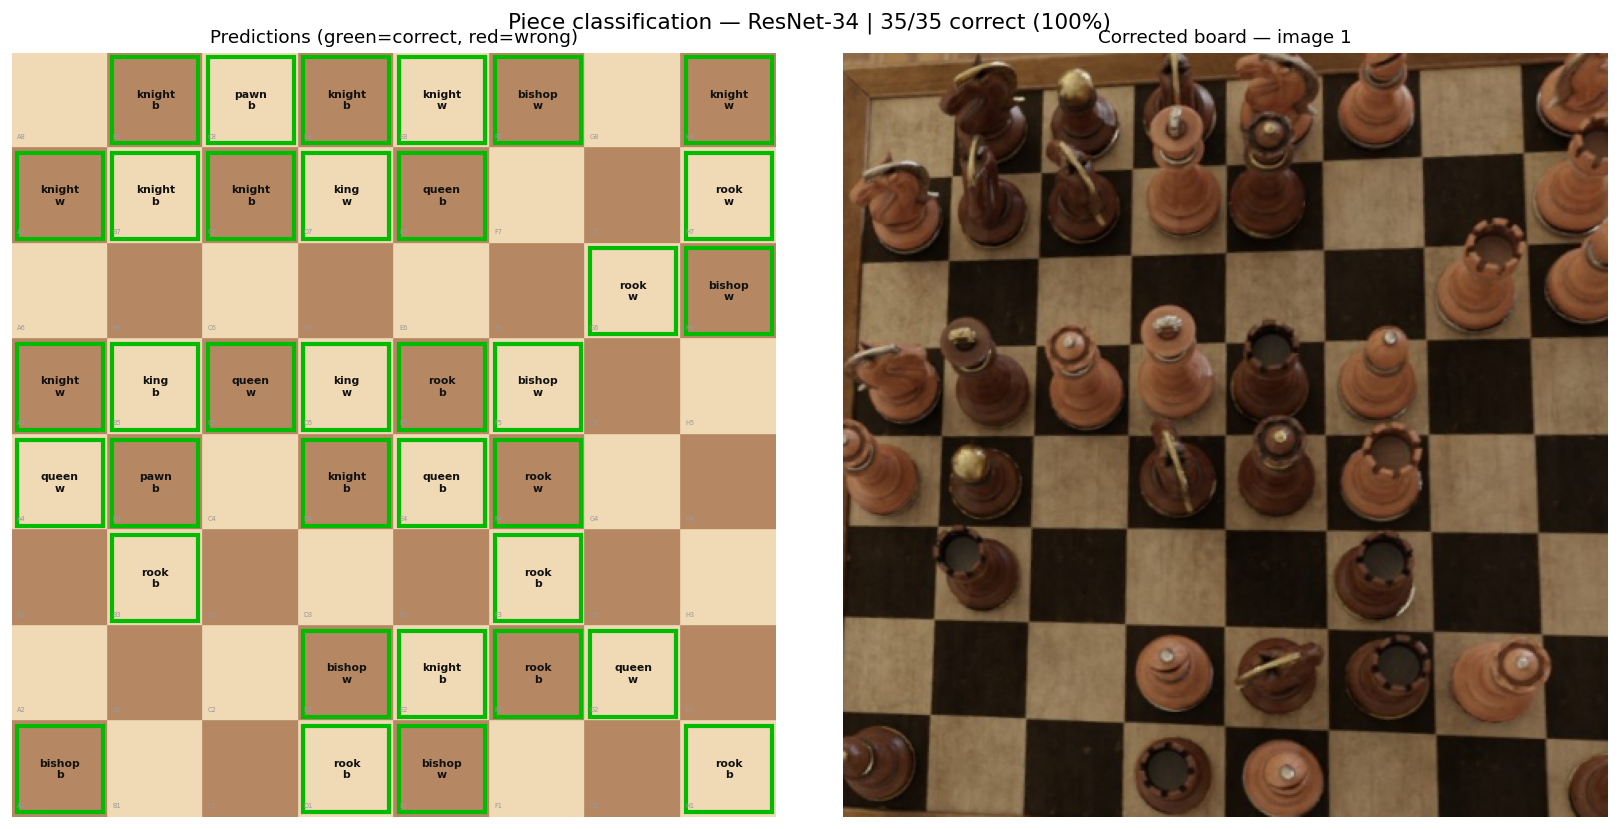
\includegraphics[width=0.55\textwidth]{../../andamento/images/15_piece_classification_result.png}
  \caption{Exemplo de leitura completa de um tabuleiro: 35/35 peças classificadas
    corretamente.}
\end{figure}

\subsection{Orientação sem gabarito e leitura de ponta a ponta}

Sobre as mesmas 60 imagens, a estimativa de orientação sem gabarito
(\texttt{detect\_board\_rotation}) apresenta \textbf{0\% de erro de eixo} --- o
tabuleiro nunca é lido girado em $90\degree$ ou $270\degree$ --- mas, como discutido na
Seção~\ref{sec:fen-jogadas}, cerca de \textbf{42\%} das leituras totalmente automáticas
ficam invertidas em $180\degree$ devido à simetria de cor do tabuleiro sob essa rotação.
Isso não é contabilizado como erro de leitura, e sim reportado explicitamente como
ambiguidade inerente, resolvida com a apresentação de duas FENs candidatas.

\subsection{Síntese}

\begin{table}[H]
\centering
\caption{Resumo por componente da pipeline.}
\small
\begin{tabular}{@{}>{\raggedright\arraybackslash}p{3.2cm}>{\raggedright\arraybackslash}p{6cm}>{\raggedright\arraybackslash}p{4.8cm}@{}}
\toprule
Componente & Abordagem & Resultado \\
\midrule
Detecção do tabuleiro & Hough + homografia & Robusto; gargalo do sistema \\
Segmentação $8\times8$ & Divisão uniforme & Exato \\
Ocupação & Votação de características (clássico) & F1 = 62,7\% (86,3\% c/ cantos GT) \\
Cor da peça & Limiar fixo de brilho HSV (clássico) & 82,5\% \\
\textbf{Tipo da peça} & \textbf{ResNet-34 --- \textit{transfer learning} + \textit{fine-tuning}} & \textbf{F1 = 91,0\%} \\
FEN + jogadas & Regras determinísticas sobre \texttt{piece\_map} & Validado em casos controlados \\
\bottomrule
\end{tabular}
\end{table}

O classificador de tipo de peça, baseado em \textit{deep learning}, é hoje a etapa mais
precisa da pipeline --- superando a precisão da detecção clássica de ocupação. O gargalo
de ponta a ponta permanece na etapa puramente geométrica de detectar os 4 cantos do
tabuleiro sob baixo contraste.

\section{Limitações e Trabalhos Futuros}
\label{sec:limitacoes}

\begin{table}[H]
\centering
\caption{Limitações conhecidas.}
\begin{tabular}{@{}p{4cm}p{4.5cm}p{5cm}@{}}
\toprule
Limitação & Impacto & Causa \\
\midrule
Material uniforme (madeira/madeira) & F1 de ocupação $\approx$ 63\% ponta a ponta & Baixo contraste peça-fundo \\
Projeção 3D de peças altas & Falsos positivos em casas vizinhas & Torre e dama ``vazam'' para casas adjacentes na foto em ângulo \\
Ambiguidade de $180\degree$ (inerente) & \textasciitilde42\% dos tabuleiros lidos invertidos (0\% de erro de eixo) & Cores do tabuleiro são simétricas sob $180\degree$; mitigado reportando as duas FENs candidatas \\
Limiares fixos (ocupação, cor) & Generalização fraca fora do dataset & Calibrados especificamente para este dataset \\
\textit{Domain shift} da CNN & Possível queda de F1 em fotos reais & Treinado apenas com imagens sintéticas do dataset \\
Ausência de sequências reais de jogo & \texttt{classify\_move} validado só em posições controladas & Dataset fornece posições independentes, não partidas contínuas \\
\bottomrule
\end{tabular}
\end{table}

\subsection{Trabalhos futuros}

\begin{itemize}[nosep]
  \item \textbf{Reforçar a detecção de cantos:} como o gargalo identificado (Seção
        \ref{sec:resultados}) é a detecção automática dos 4 cantos do tabuleiro,
        investigar detectores mais robustos (ex.: RANSAC sobre as retas de Hough,
        ajuste com restrição de checkerboard) deve trazer o maior ganho de F1 de ponta
        a ponta.
  \item \textbf{Reduzir falsos positivos de ocupação:} calibrar limiares por imagem
        (adaptativos) em vez de globais, ou combinar as quatro características por um
        classificador aprendido em vez de votação por maioria fixa.
  \item \textbf{Validação em jogo real:} testar a pipeline com fotos de um tabuleiro
        físico real, com iluminação e materiais fora da distribuição do dataset
        sintético, para quantificar o \textit{domain shift} da CNN.
  \item \textbf{Sequências reais de jogo:} coletar ou gerar uma sequência contínua de
        posições de uma mesma partida para validar \texttt{classify\_move} em condições
        reais, incluindo o efeito acumulado de pequenos erros de leitura entre frames.
  \item \textbf{Distribuição do modelo treinado:} publicar os pesos da ResNet-34
        (\texttt{.pth}) em um local versionado com download automático via
        \texttt{setup.py}, eliminando a necessidade de retreinar para reproduzir os
        resultados.
\end{itemize}

\section{Conclusão}

Este trabalho implementou uma pipeline completa de leitura automática de tabuleiros de
xadrez, combinando visão computacional clássica --- para geometria do tabuleiro,
ocupação e cor --- com \textit{transfer learning} de uma ResNet-34 para a única etapa em
que a abordagem clássica se mostrou insuficiente: a classificação do tipo de peça. A
pipeline cobre o problema de ponta a ponta, da fotografia bruta em perspectiva até a
notação FEN completa (seis campos) e a inferência de jogadas, incluindo casos especiais
como captura, roque, \textit{en passant} e promoção.

Os resultados quantitativos mostram que o classificador de tipo de peça baseado em
\textit{deep learning} (F1 = 91,0\%) é hoje a etapa \textbf{mais precisa} do sistema,
superando a etapa puramente clássica de detecção de ocupação (F1 = 62,7\% ponta a ponta,
86,3\% isolando o erro de detecção de cantos). Esse resultado identifica claramente o
gargalo do sistema: não é a classificação de tipo de peça, e sim a detecção geométrica
robusta dos 4 cantos do tabuleiro sob baixo contraste --- o ponto de maior retorno para
trabalho futuro.

O projeto também documentou explicitamente um limite \textbf{intrínseco} da leitura a
partir de uma única imagem --- a ambiguidade de orientação de $180\degree$ causada pela
simetria de cor do tabuleiro --- em vez de tratá-lo como um bug a esconder, reportando as
duas FENs candidatas sempre que a leitura é totalmente automática.

De forma mais ampla, o trabalho demonstra que combinar visão clássica e \textit{deep
learning}, cada uma aplicada onde é mais forte, produz uma pipeline mais robusta e mais
interpretável do que qualquer uma das duas abordagens isoladamente: a geometria clássica
permanece transparente e auditável, enquanto a rede neural resolve apenas o
sub-problema --- reconhecimento fino de forma sob baixo contraste --- para o qual
descritores clássicos não bastaram.

\section{Links do Projeto}
\label{sec:links}

\begin{itemize}
  \item \textbf{Dataset:} \textit{Synthetic Chess Board Images} (Kaggle, thefamousrat,
        licença CC0) --- \url{https://www.kaggle.com/datasets/thefamousrat/synthetic-chess-board-images}
  \item \textbf{Código-fonte (GitHub):} \url{https://github.com/daviludvig/classical-cv}
  \item \textbf{Checkpoint do modelo (ResNet-34 treinada, \texttt{.pth}):}
        \todolink{publicar os pesos treinados (GitHub Releases / Hugging Face) e
        inserir o link direto de download aqui}
  \item \textbf{Apresentação (Google Slides):}
        \todolink{publicar \texttt{docs/final/apresentacao.md} (Marp) como Google
        Slides e inserir o link de compartilhamento aqui}
  \item \textbf{Vídeo (YouTube):}
        \todolink{gravar, exportar em H.265 e enviar ao YouTube; inserir o link aqui}
  \item \textbf{Poster (PDF, A1):} anexado ao final deste documento (Anexo~\ref{sec:poster}).
\end{itemize}

\section{Declaração de Uso de Inteligência Artificial Generativa}
\label{sec:declaracao-ia}

Em conformidade com as diretrizes da disciplina para a entrega do trabalho final,
declaramos o uso pontual de Inteligência Artificial Generativa (ferramenta:
\textbf{Claude AI}, Anthropic) como suporte durante o desenvolvimento do código.
Abaixo detalhamos as áreas específicas onde a ferramenta foi utilizada, os prompts
empregados e a explicação do funcionamento do código gerado, demonstrando compreensão
da lógica integrada ao projeto --- e não o uso de uma "caixa preta".

\subsection{Cálculo de métricas (F1-score, precisão e recall)}
\label{sec:declaracao-ia-metricas}

\textbf{Arquivo afetado:} \texttt{scripts/eval\_metrics.py}

\begin{quote}
\itshape
``Como posso implementar uma função em Python usando NumPy para calcular a Matriz de
Confusão (Verdadeiros Positivos, Falsos Positivos e Falsos Negativos), a Precisão, o
Recall e o F1-Score comparando dois arrays booleanos 8x8 (um com a predição de
ocupação do tabuleiro e outro com o ground truth)? Preciso que o código evite o erro
de `divisão por zero'.''
\end{quote}

\textbf{Explicação do código gerado:} o trecho gerado e adaptado por nós calcula o
F1-score da detecção de ocupação do tabuleiro:
\begin{enumerate}[nosep]
  \item \textbf{Verdadeiros Positivos (TP):} comparação elemento a elemento entre a
        matriz de predição e a matriz de \textit{ground truth} (GT), \texttt{(pred == 1)
        \& (gt == 1)} --- casas de fato ocupadas que o modelo acertou.
  \item \textbf{Falsos Positivos (FP):} \texttt{(pred == 1) \& (gt == 0)} --- casas que o
        modelo marcou como ocupadas, mas o GT indicava vazias.
  \item \textbf{Falsos Negativos (FN):} \texttt{(pred == 0) \& (gt == 1)} --- peças que o
        modelo não detectou.
  \item \textbf{Fórmulas:} Precisão $= TP / (TP + FP)$; Recall $= TP / (TP + FN)$;
        F1 $= 2 \cdot (\text{Precisão} \cdot \text{Recall}) / (\text{Precisão} +
        \text{Recall})$. O código inclui um termo mínimo ($\epsilon = 10^{-9}$) somado
        ao denominador --- necessário para evitar divisão por zero no caso extremo de um
        tabuleiro inteiro ser lido como vazio, o que zeraria o denominador da precisão.
\end{enumerate}

\subsection{Visualização de resultados (bounding boxes com Matplotlib)}
\label{sec:declaracao-ia-viz}

\textbf{Arquivo afetado:} notebooks de visualização e geração de figuras do relatório.

\begin{quote}
\itshape
``Escreva um trecho de código usando Matplotlib que pegue uma imagem de um tabuleiro
de xadrez 480x480 retificado, faça um loop para dividi-lo em um grid de 8x8 (60x60
pixels por casa) e desenhe `bounding boxes' verdes nas casas onde o modelo acertou e
vermelhas nas casas onde o modelo errou. Como desenho esses retângulos vazados em cima
da imagem original?''
\end{quote}

\textbf{Explicação do código gerado:} usamos a IA para acelerar a geração de código
\textit{boilerplate} de plotagem (não de processamento de imagem), usado exclusivamente
para gerar as figuras do relatório:
\begin{enumerate}[nosep]
  \item Inicialização de figura e eixo (\texttt{fig, ax = plt.subplots()}), com a imagem
        de fundo (tabuleiro retificado) exibida via \texttt{ax.imshow()}.
  \item Loop duplo aninhado (\texttt{for i in range(8)}, \texttt{for j in range(8)})
        percorrendo o grid 8$\times$8.
  \item Coordenada do canto superior esquerdo de cada casa obtida multiplicando os
        índices pelo tamanho em pixels (\texttt{x = j * 60}, \texttt{y = i * 60}).
  \item Cada casa é desenhada com um objeto
        \texttt{matplotlib.patches.Rectangle}, recebendo posição, largura, altura, cor
        da borda e \texttt{facecolor='none'}. É esse último parâmetro que garante que a
        caixa fique vazada, sem cobrir a peça na imagem.
  \item A cor é definida dinamicamente a partir da nossa matriz de comparação
        predição~$\times$~\textit{ground truth}: verde em caso de acerto, vermelho em
        caso de erro. Cada retângulo é adicionado à figura com \texttt{ax.add\_patch()}.
\end{enumerate}


\printbibliography

\clearpage
\section*{Anexo: Poster do Trabalho (A1)}
\label{sec:poster}
\addcontentsline{toc}{section}{Anexo: Poster do Trabalho (A1)}
\includepdf[pages=-]{../poster.pdf}

\end{document}
